\chapter{微积分 - 偏导数-方向导数}

\begin{figure}[ht]
  \centering
  \includegraphics[width=1\textwidth]{asset/茶桁的 AI 秘籍_Math_11.png}
\end{figure}

\newpage

我们上节课学习了链式法则, 本节课, 我们要学习「偏导数」和「方向导数」. 

\section{偏导数}

偏导数在导论课里面也提到过. 偏导数针对多元函数去讲的. 

多元函数是什么, 我们拿个例子来看: 

\begin{align*}
  \mbox{多元函数: }y = f(x_1, x_2, ..., x_n)
\end{align*}

就是包括$x_1,  x_2,  ...,  x_n$这么多自变量在$f$的映射作用才能得到这么一个$y$. 所以, 它和一元函数的导数的情况不太一样, 它的因变量相对于每一个自变量都有一个导数, 是针对于每一个单独自变量所求出来的导数, 所以称为偏导数. 

偏导数的形式如下: 

\begin{align*}
  \frac{\partial y}{\partial x_1},  \frac{\partial y}{\partial x_2},  ...,  \frac{\partial y}{\partial x_n} \quad \mbox{或者} \quad f_{x_1},  f_{x_2},  ...,  f_{x_n}
\end{align*}

其实和导数一样读作\(dy\),  但是因为需要区别导数和偏导数, 所以就用了\(\partial\), 在 Latex 中, 写作\pyth{\partial}.

偏导数还可以使用函数本身, 再在右下角加上相对应的自变量来表示. 就比如 $y$ 相对于 $x_1$ 的偏导数, 就可以用$f_{x_1}$来表示. 

不要看它好像很复杂, 这么多的自变量, 我们该怎么样去处理啊?本质上它仅仅是\textit{因为是一个多元函数的导数, 所以才多了一个“偏”字, 而且其求解的过程其实和导数没有任何区别}. 

打个比方说, 求 $y$ 相对于 $x_1$ 的偏导数, 我把$x_2, ..., x_n$ 都看作是常数, 就不用去管它, 只需要关注 $x_1$ 就行了, 其定义的式子也可以显现出这一点: 

\begin{align*}
  \frac{\partial f(x, y)}{\partial x}  = f_x(x, y) = \lim_{h \to 0} \frac{f(x+h, y) - f(x, y)}{(x+h)-x}
\end{align*}

$\frac{\partial f(x, y)}{\partial x}$ 这是一个二元函数,求关于 $x$ 偏导数, 可以写成 $f_x(x, y)$ 这种形式,定义就是说这里虽然是有两个量,但是 $y$ 我不关心, $y$ 就是 $y$ , 我只关心 $x, x+h$, 两者无限逼近的这么一个过程. 

所以,大家可以发现如果把 $y$ 给拿掉,不就是我们求导的过程吗. 

所以偏导数和导数一模一样, 没有任何区别. 

那下面这个例子, 我们在导论课中就已经见到过了,再拿出来也是带大家回顾一下:

\begin{align*}
  \mbox{例: } & \mbox{求多元函数} y = f(x_1, x_2) = x_1^2 + x_1x_2+sinx_2\mbox{的偏导数及导数. }\\ \\
  \mbox{解:  }& \frac{\partial y}{\partial x_1} = 2x_1 + x_2 \\
  & \frac{\partial y}{\partial x_2} = x_1 + cos x_2
\end{align*}

只要导数会求, 偏导数其实就没什么问题. 只要能理解这么个东西怎么求, 就基本上可以和偏导数这一课说 goodbye. 

比如我们给出多元函数 $x_1^2 + x_1x_2+sinx_2$ 的偏导数. 那我们怎么求呢?

首先求 $y$ 关于 $x_1$ 的偏导的时候其他的自变量就看做常数, 所以第一项 $x_1^2$ 就求出 $2x_1$, 第二项$x_1x_2$ 就相当于一个常数乘上$x_1$, 常数就是$x_2$. 

然后第二个式子,是 $\frac{\partial y}{\partial x_2}$ 等于什么? 首先我们还是先来看下第一项, 第一项有没有 $x_2$ 呢?没有. 没有的话这一项就相当于一个常数了,对常数求导结果就是 0. 为什么对常数求导结果是 0 我们之前有讲过, 因为常数不管输入是多少, 输出永远是一个恒定的量, 在几何图像上面显示出来就是没有任何变化,就是一条水平线, 所以对常数求导他的导数是 0. 

好, 第一项没了. 第二项是$x_1x_2$, 相当于一个常数乘 $x_2$, 常数是$x_1$, 所以这里保留下来. $sinx_2$ 求导就是$cosx_2$. 

多说两句题外话, 偏导数到了实际应用里有什么关联呢?因为我们在人工智能里面, 它不是这种一对一的一元函数关系, 是多元函数关系. 比如说 $sinx, cosx$, 可能不仅产生 $y_1$, 在不同的映射法则之下甚至可能产生 $y_2, y_3$. 所以我们需要了解神经网络里面不是一元函数的导数, 更有可能的是偏导数, 然后逐层反向传播, 这就是偏导数的一个应用. 

\section{方向导数}

我们再来看一下方向导数. 方向导数的内容可能也会稍微复杂一点, 但是因为考虑到课程体系, 有些东西我觉得确实是没办法去删减. 所以在这里也给大家把这部分知识也给讲上. 

我们刚才说的偏导数都是沿着自变量方向的. 比如 $\frac{\partial y}{\partial x}$, 都是沿着自变量方向的, 如图\ref{fig:img12_1}: 

\begin{figure}[ht]
  \centering
  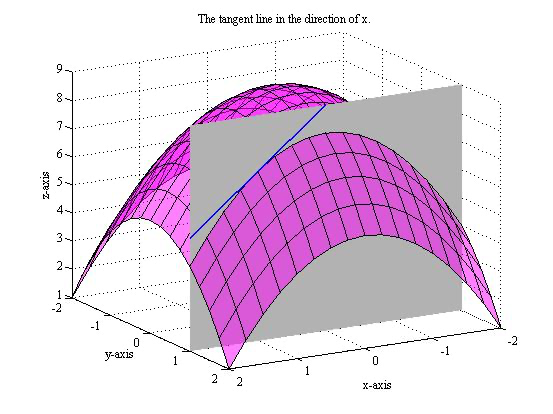
\includegraphics[width=0.5\textwidth]{asset/20230901095029.png}
  \caption{}
  \label{fig:img12_1}
\end{figure}

在这张图里, $x$ 和 $y$ 就是自变量, $z$ 是函数值. 在这种情况下, 偏导数可以沿着什么呢?比如说沿着 x 的方向把二元函数曲面给截出来, 就如图中这样, 类似一个抛物线的形状. 所以, 偏导数都是沿着自变量的方向. 

那又有一个问题了: 我们能不能沿着任意方向去求导数呢?非得沿着 $x$ 还有沿着 $y$ 去求吗? 确实这是一个好问题. 先说结论, 是可以沿着任意方向求的. 我们来看图 \ref{fig:img12_2}: 

\begin{figure}[ht]
  \centering
  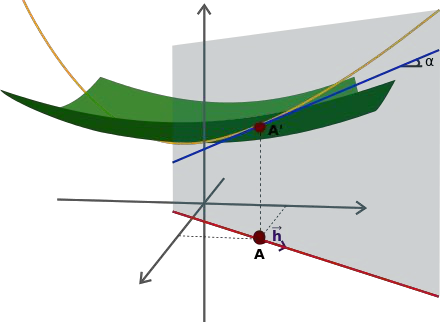
\includegraphics[width=0.5\textwidth]{asset/20230901095643.png}
  \caption{}
  \label{fig:img12_2}
\end{figure}

这张图在绿色这个曲面上面就不一定非得沿着 $x$ 或者 $y$ 方向了. 可以沿着红线的方向, 任意的都可以求. 

又来问题了. 在一元函数里面自变量它在函数曲线上只能沿着两个方向去移动. 我们继续来看图 \ref{fig:img12_3}. 这张图上, 我们在抛物线上 X 轴左侧随意取一点, 这个点坐落在抛物线上, 要么往上要么往下, 往上就对应着 x 减小, 往下对应 x 增大的这么一个方向. 它只能沿着这两个方向,没其他选择了. 

\begin{figure}[ht]
  \centering
  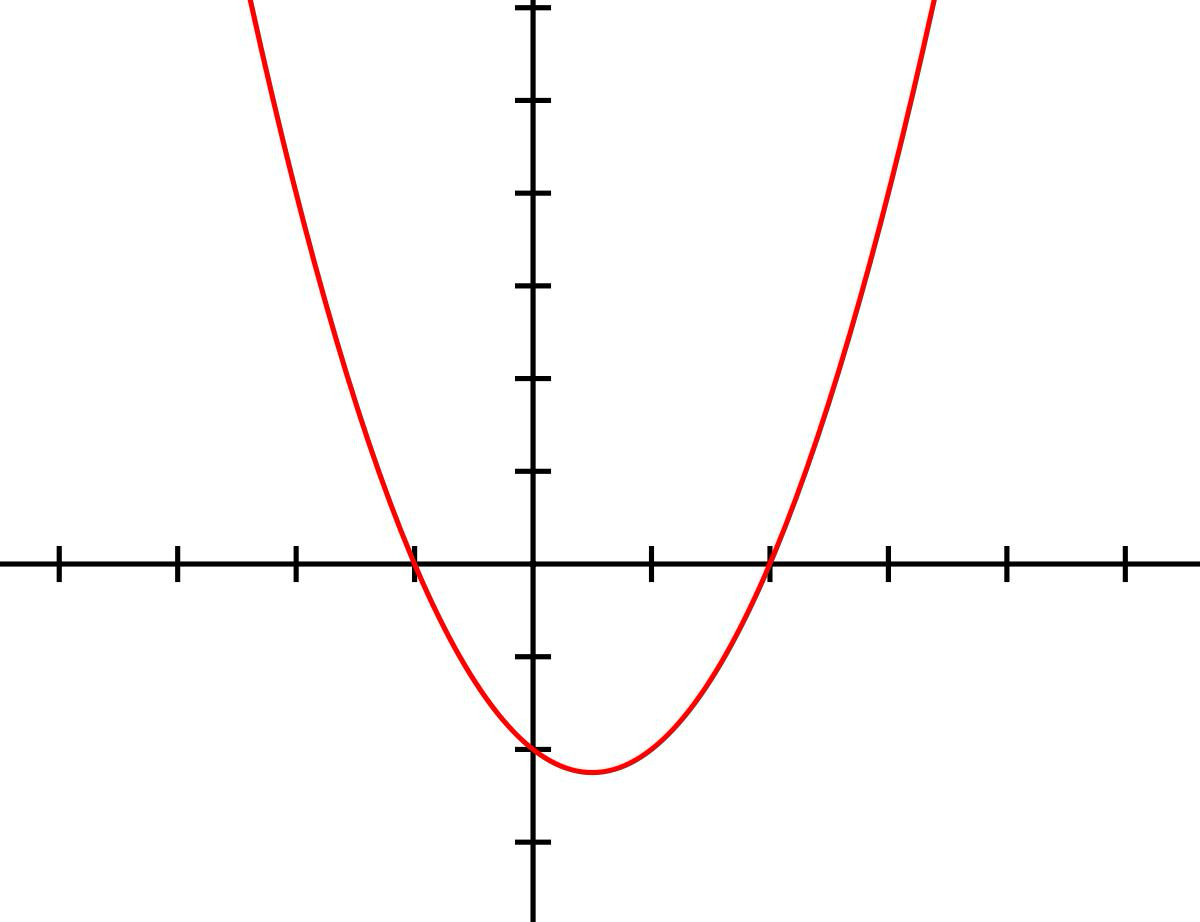
\includegraphics[width=0.5\textwidth]{asset/20230901095921.png}
  \caption{}
  \label{fig:img12_3}
\end{figure}

但是\textbf{在多元函数中,自变量在函数曲面上可以沿着无穷多个方向去移动}. 来继续看一下上面的图\ref{fig:img12_2}: 

就像图\ref{fig:img12_2}里, 在曲面上面任取一个方向, 比如说把红线再稍微转一点它就是一个新的方向,再转一点呢,又是一个新的方向. 

所以在\textbf{多元函数里面,函数的变化不仅和你移动距离有关}, 也就是说不仅和$\partial y$有关, 它\textbf{还和你选择的方向有关}. 

如何得来呢?我们来看: 

\begin{align*}
  \frac{\partial z}{\partial l} \Bigg \vert _p = \lim_{p' \to p} \frac{f(P') - f(P)}{|P'P|}
\end{align*}

对于一个函数 $z=f(x,y)$, 对于函数而言, 我们在这里求它偏导的话就是 $\frac{\partial z}{\partial x}$ 或者 $\frac{\partial z}{\partial y}$, 但是这里我不是比上$\partial x$ 或者$\partial y$了, 而是比上$\partial l$, $l$ 代表着一个方向, 在图\ref{fig:img12_4} 中其实就是红线, 坐落在$x, y$轴线形成的平面上的那一根红线,它代表的一个方向. 

\begin{figure}[ht]
  \centering
  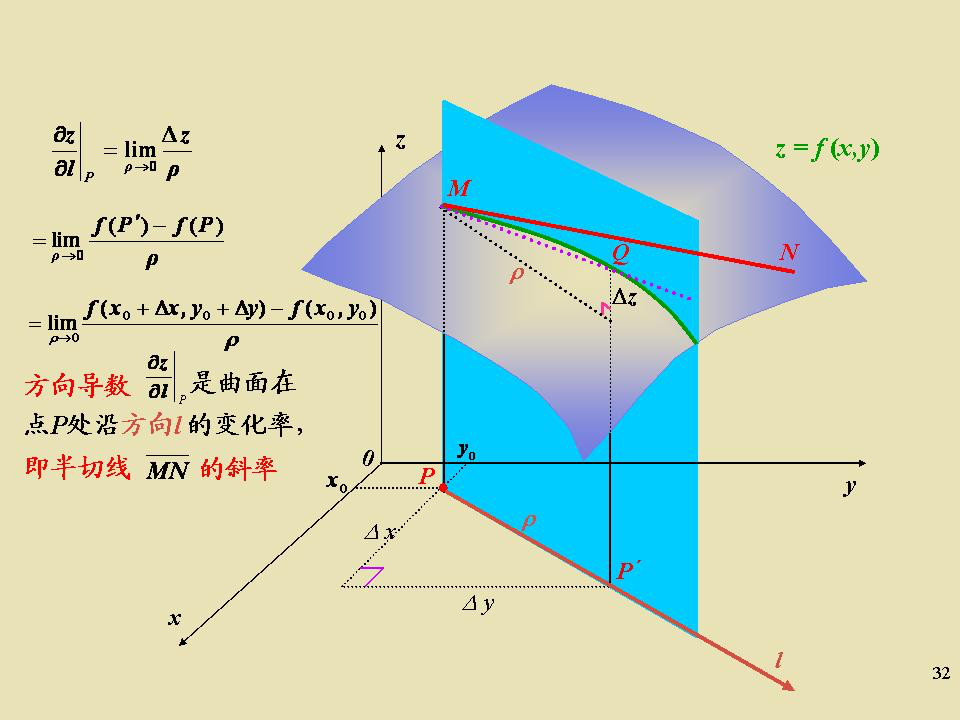
\includegraphics[width=0.8\textwidth]{asset/20230901103919.png}
  \caption{}
  \label{fig:img12_4}
\end{figure}

我们来看一下式子,方向导数的定义式其实和偏导数很类似,只不过它就是沿着 l. 我们看到这个图像,它很复杂,是一个二元函数. $x$ 和 $y$ 都是自变量. 跟着我的步骤一步一步, 别自己跑丢了. 

$z$ 是 $x, y$ 的一个函数值. 就像图中绿色字体标出来的一样,$z = f(x, y)$, 所以自变量就可以在 $x, y$ 平面内任意取中一点, 然后在 $f$ 的映射规则下得到一个 $z$ 值, 也就得到竖值方向, 也就是 $z$ 轴上面的一个值, 形成一个曲面. 

当我们现在沿$l$方向去求它方向导数的时候,其实我们还是用无限逼近的原理去做. 

首先, 我们取两个点, 先取点 $P$, 坐标是 $x_0, y_0$, 然后我们取另外一个点 $P'$,$P'$ 对应着曲面上的点是 $Q$ 点, $P$ 点对应的是 $M$ 点. $P$ 和 $P'$ 对应着我们自变量的取值, $M$ 和$Q$ 是我们图像上面的点. 因为 $M$ 和 $Q$ 是有 $z$ 坐标的, 而$P$ 和 $P'$ 是没有的. 

我们就来看一下 $P$ 和 $P'$, 当 $P'$ 不断的向 $P$ 靠近,不断的逼近的时候, 它们中间的长度也趋向于 0. 则 $M$ 和 $Q$ 也是趋向于 0 的. 

在过程当中就采取一个类似类比的思想, 就是我在这里把 $P, P'$ 作$\partial x$, 把这两点的长度看作是 $\partial x$, 也就是我们导数里面的 $\partial x$.  $f(P')$ 其实就是 $Q$ 点在 $z$ 轴上面的值. 再减去 $M$ 点对应的 $z$ 轴上面值, 其实也就是 $f(P)$, 也就是 $f(P') - f(P)$. 

我们定义式, 就可以写成 $\lim_{p' \to P} \frac{f(P') - f(P)}{|P'P|}$ 这个式子. 

大家可以和我们导数的定义式类比一下, 同样一个极限符号, 其中一个点向另外一个点无限逼近, 分母是一个$\partial x$. 在这里的$\partial x$ 就是 $(P,P')$ 的长度,写作 $|P'P|$, 它们函数值之差就是 $f(P') - f(P)$, 也就是区域点的 $z$ 座标值减去 $M$ 点的 $z$ 座标值. 令 $l$ 的方向余弦为: 

\begin{align*}
  (cos \alpha, cos \beta, cos \gamma)
\end{align*}

这里还需要一个概念,叫做 $l$ 的一个「方向余弦」. 方向余弦是什么东西呢?稍后我们就会讲到,先接着之前的继续说: 当我们在这里把 $f(P') - f(P)$ 写出来之后, 它具体的代表其实是下面的这么一行公式: 

\begin{align*}
  \lim_{P \to 0} \frac{f(x_0 + \Delta x, y_0+\Delta y) - f(x_0, y_0)}{P} \\
\end{align*}

$P'$ 相对于 $P$ 点, 它们俩之间的差是怎么得到的呢? 是不是$x_0$ 再加上沿 X 轴上的一节长度 $\Delta x$, $y_0$ 加上沿 Y 轴的一段长度 $\Delta y$, 就到达 $P'$ 了. 

也就是说, $P'$ 的坐标就是 $x_0 + \Delta x, y_0+\Delta y$. 因为自变量是两个 $x, y$, 所以函数里面就是 $f(x_0 + \Delta x, y_0+\Delta y) - f(x_0, y_0)$. 

所以, 方向导数 $\frac{\partial z}{\partial l}$, 是曲面在$P$ 点处代表着沿 $\partial l$, 也就是沿着红线方向的变化率. 之前的偏导数要么沿着 $x$ 方向,要么沿着 $y$ 方向. 现在就很自由了, 想沿哪个方向就沿哪个方向, 只要这个方向能求导. 所以, 我沿 l 方向就被称为沿着 $l$ 方向的方向导数. 也就是半切线$\overline {MN}$ 的一个斜率. 

$\overline {MN}$ 是怎么得到的? 就是 $P'$ 无限逼近 $P$ 的过程当中, $Q$ 也无限逼近 $M$, 就像我们二次函数里面的例子一样,这两个点无限逼近到一块去之后,在 $M$ 点重合,那 $M$ 点这里就有一条切线. 切线的斜率就是方向导数的数值. 也就是它的几何意义. 

大家怎么样去理解呢, 最好是把它和导数那一部分去做一个类比的理解. 分母就是 $\partial x$, 就是自变量的一个差值. 分子部分是函数值的一个差异. 

\subsection{方向余弦}

我们刚才说到有个概念叫「方向余弦」. 方向余弦在接下来的求导过程当中需要用到, 所以我们要了解一下什么是方向余弦. 

余弦大家在初中就接触过, 初中数学就有上过正弦余弦,这里就是在那个基础之上. 它的定义为: 

\begin{newquotation}
  向量与三个(或两个)坐标轴之间的角度的余弦: $cos \theta_1, cos \theta_2, cos \theta_3$
\end{newquotation}

我们来看图\ref{fig:img12_5}: 

\begin{figure}[ht]
  \centering
  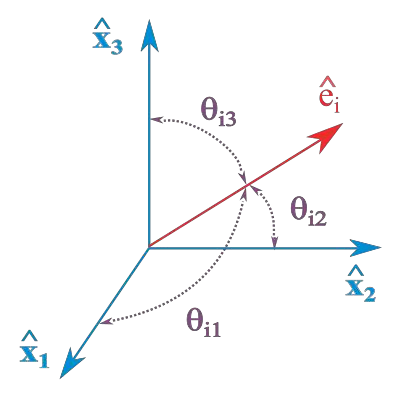
\includegraphics[width=0.5\textwidth]{asset/20230901155252.png}
  \caption{}
  \label{fig:img12_5}
\end{figure}

这个向量和这三个坐标轴都会有一个夹角,分别是 $\theta_1, \theta_2, \theta_3$, 如果是平面直角坐标的话, 那它只会和两个坐标轴有角度: $x$ 轴 $y$ 轴, 就没有 $z$ 轴. 如果是三维的情况, 它就三个夹角的余弦值, 组合到一起就叫做「方向余弦」, 分别是$cos \theta_1, cos \theta_2, cos \theta_3$, 这三个余弦的平方和等于 1. 

如果是在平面直角坐标系里面, 两个值的情况很好理解. 因为我们只考虑这 $x, y$ 平面, 而不考虑有 $z$ 轴. 那我们现在就只考虑平面: 比如, 这里有一个向量, 它和 x 轴夹角是 30 度, 那和 y 轴夹角就肯定是 60 度. $cos30^\circ$ 应该是等于 $\frac {\sqrt 3}{2}$, $cos 60^\circ$ 是等于$\frac{1}{2}$, $(\frac{\sqrt 3}{2})^2 + (\frac{1}{2})^2$, 算一下结果就是等于 1. 不管是二维还是三维式子, 平方和等于 1 是始终成立. 

\subsection{投影}

这里又需要多出一个概念叫「投影」, 立体向量 $\vec e$ 在 $x_1$ 方向上的投影就是其自己的本身的长度乘以它和相应的坐标轴之间夹角的余弦值. 如下: 

\begin{itemize}
  \item 向量 $\vec e$ 在 $x_1$ 方向上的投影为: $|\vec e| cos \theta_1$ 
  \item 向量 $\vec e$ 在 $x_2$ 方向上的投影为: $|\vec e| cos \theta_2$ 
  \item 向量 $\vec e$ 在 $x_3$ 方向上的投影为: $|\vec e| cos \theta_3$ 
\end{itemize}

就像一束光打到墙上一样. 本来这个向量箭头非常长, 但是因为有一个角度, 它投射在坐标的某一个方向上, 垂直于某一个方向的时候其实是有一个压缩的, 我们就把它叫做投影. 这和我们生活当中的投影也是非常类似. 所以投影值肯定是比你原来向量长度要小. 

因为三角函数值不可能大于 1, 所以肯定不会超过原来向量的长度. 这个其实也是初中数学的内容. 

那我们现在就知道了方向余弦是怎么一回事了. 就是向量和坐标轴之间的一个夹角的余弦组合在一起. 

\subsection{继续讲方向导数}

还是回过去看图\ref{fig:img12_4}, 我们说令 l 的方向余弦为: ($cos \alpha , cos \beta$), 在图中我们并没有表示出$\alpha$, 其实就是 $l$ 和 $x$ 轴之间的夹角, $\beta$ 就是$l$ 和 $y$ 轴之间的夹角. 

看到这里, 可能有的小伙伴要问了, 三维里面它应该是三个夹角, 那为啥在这里没有说它和 $z$ 轴的夹角?这是因为虽然它图像三维的, 但是自变量只有两个. $z$ 轴其实是它的函数值, 不是自变量, 所以我们就不考虑 $z$ 轴, 只考虑平面, 得到方向余弦只考虑 $x, y$ 这两个坐标轴的一个夹角. 

然后令 $t = |P'P|$, 令它的长度就是 $\rho$, 图里标示的$\rho$. 所以点 $P'$ 可以表示成下面这样: 

\begin{align*}
  x_{P'} = x_p + t cos \alpha, y_{p'} = y_p + t cos \beta
\end{align*}

其实就是股股定理, 这里应该不难理解. 

接下来改写一下形式, 我们已经知道 $l$ 方向的导数 $\frac{\partial z}{\partial l} \Bigg \vert _p$ 可以是函数的变化量除以自变量的变化量就是 $\frac{\Delta f}{t}$, $t$就是这一节长度. 然后进一步去写:

\begin{align*}
  \frac{\partial z}{\partial l} \Bigg \vert _p & = \lim_{t \to 0}\frac{\Delta f}{t} \\
  & = \lim_{t \to 0} \frac{f_x\Delta x + f_y \Delta y + o(t)}{t}
\end{align*}

$\Delta f$是分成两个方向的,一个是$x$方向,一个是$y$方向. 在这里涉及到了一个概念叫做「全微分」,这里我没有把它拿出来再说了,我怕加太多内容大家就更云里雾里的了. 所以大家就这样去理解: 因为是有两个自变量,所以肯定函数值发生变化来源于两个方面的贡献,一个是$x$方向一个是$y$方向. 

这里可以把$\Delta f$写成$f_x\Delta x + f_y \Delta y + o(t)$, 用$\Delta$表示是因为是要取一个极限, 所以我们不用$\delta$, 用$\Delta$表示增量. 就是关于$x$的偏导数乘上$x$的增量, 写成$f_x\Delta x$. 

大家可以注意到我们在之前说到微分的时候,就说到$df(x) = f'(x)dx$ , 也就是$f(x)$的导数乘上自变量的变化率,就等于函数的变化率$df(x)$. 就是微分的概念. 

所以这里其实我们也是做同样的处理,只不过它分成两个方向,$x$方向和$y$方向. $f_x(\Delta x)$对应着 x 方向对于函数增量的一个贡献,还有 y 方向的增量的贡献$f_y \Delta y$.  

后面的$o(t)$代表关于 t 的一个无穷小量. 在取极限的情况下,这项就可以忽略掉,我们的重点可以不用放在这一块. 

在之后,我们再去做一个转换:

\begin{align*}
  \frac{\partial z}{\partial l} \Bigg \vert _p & = \lim_{t \to 0}\frac{\Delta f}{t} \\
  & = \lim_{t \to 0} \frac{f_x\Delta x + f_y \Delta y + o(t)}{t} \\
  & = \lim_{t \to 0} \frac{t(f_xcos \alpha + f_y cos\beta + o(t))}{t} 
\end{align*}

在这里, $\Delta x$其实就是$t cos \alpha$, $\Delta y$也就是$t cos \beta$. 所以在这里都统一改写一下,那么我们最终会得到一个怎样的结果呢?我们最终会得到下面这样的一个结果: 

\begin{align*}
  \frac{\partial z}{\partial l} \Bigg \vert _p & = \lim_{t \to 0} \frac{t(f_xcos \alpha + f_y cos\beta + o(t))}{t} \\
  & = f_x cos \alpha + f_y cos \beta \\
  & = \begin{bmatrix} f_x \quad f_y  \end{bmatrix} \begin{bmatrix} cos  \alpha \\ cos \beta \end{bmatrix}
\end{align*}

$f$在$x$上的偏导数乘上$cos \alpha$加上 f 在 y 方向上的偏导数乘上$cos\beta$: ($f_x cos \alpha + f_y cos \beta $). 

如果用向量的形式来写就是: 

\begin{align*}
  \begin{bmatrix} f_x \quad f_y  \end{bmatrix}
  \begin{bmatrix} cos \alpha \\ cos \beta \end{bmatrix}
\end{align*}

这里第一个向量是一个行向量, 是关于两个自变量的一个偏导数. 第二个是方向余弦. 应该还记得线性代数吧?我们在导论课里面上的那部分内容, 一个行向量一个列向量. 在这里, $\begin{bmatrix} f_x \quad f_y \end{bmatrix}$ 就是「梯度」, 用$\nabla f$ 来表示. $\begin{bmatrix} cos \alpha \\ cos \beta \end{bmatrix}$ 是$l$方向的方向余弦, 且其长度为 1, 用$\vec l$ 表示. 

最终$l$方向上的方向导数就变成了我们所说的梯度和$l$方向的方向余弦的一个向量乘积, 换句话说, 就是函数$f(x)$在$l$方向上的导数就是在该点的梯度和$\vec l$的内积. 

这两个向量乘在一起,什么时候乘积最大呢?只有他们同向的时候乘积最大. 也就是说当$\nabla f$和$\vec l$方向一致时,它们的内积最大,就是方向导数最大. 所以其实间接证明了一个美妙的结论: 梯度的方向是函数变化最快的方向. 

至于什么叫做梯度, 留到下节课来讲. 